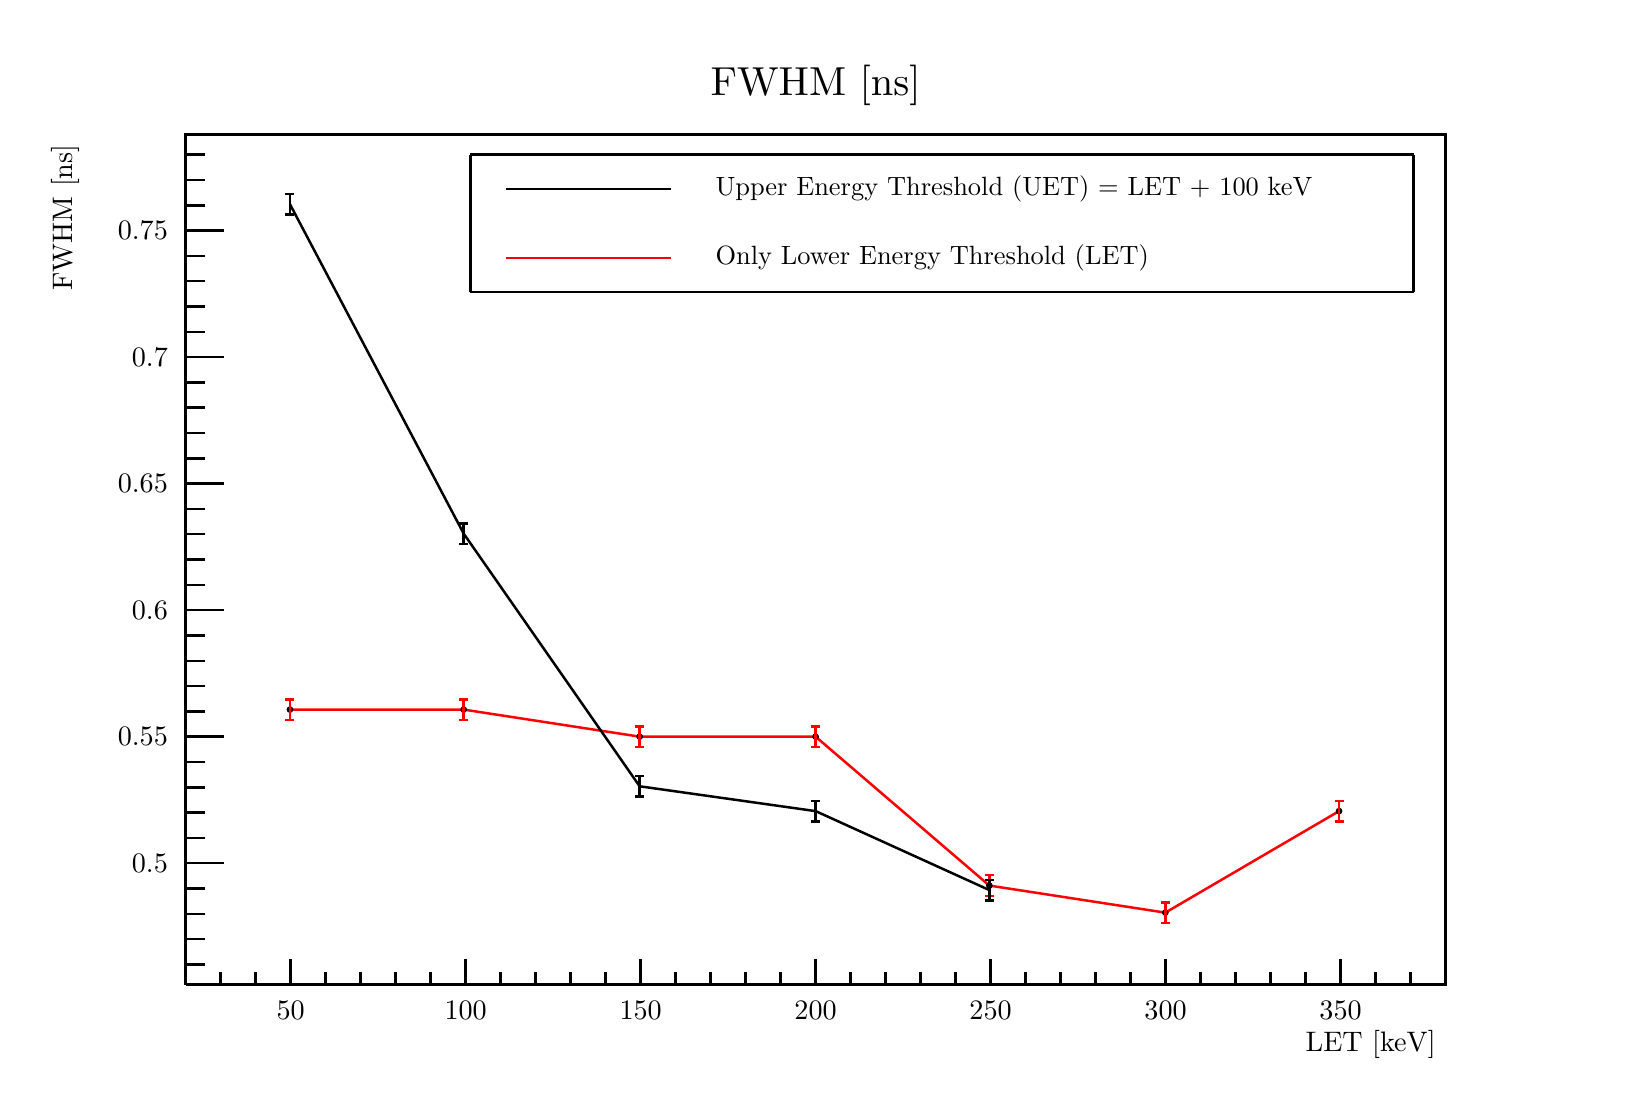
\begin{tikzpicture}
\pgfdeclareplotmark{cross} {
\pgfpathmoveto{\pgfpoint{-0.3\pgfplotmarksize}{\pgfplotmarksize}}
\pgfpathlineto{\pgfpoint{+0.3\pgfplotmarksize}{\pgfplotmarksize}}
\pgfpathlineto{\pgfpoint{+0.3\pgfplotmarksize}{0.3\pgfplotmarksize}}
\pgfpathlineto{\pgfpoint{+1\pgfplotmarksize}{0.3\pgfplotmarksize}}
\pgfpathlineto{\pgfpoint{+1\pgfplotmarksize}{-0.3\pgfplotmarksize}}
\pgfpathlineto{\pgfpoint{+0.3\pgfplotmarksize}{-0.3\pgfplotmarksize}}
\pgfpathlineto{\pgfpoint{+0.3\pgfplotmarksize}{-1.\pgfplotmarksize}}
\pgfpathlineto{\pgfpoint{-0.3\pgfplotmarksize}{-1.\pgfplotmarksize}}
\pgfpathlineto{\pgfpoint{-0.3\pgfplotmarksize}{-0.3\pgfplotmarksize}}
\pgfpathlineto{\pgfpoint{-1.\pgfplotmarksize}{-0.3\pgfplotmarksize}}
\pgfpathlineto{\pgfpoint{-1.\pgfplotmarksize}{0.3\pgfplotmarksize}}
\pgfpathlineto{\pgfpoint{-0.3\pgfplotmarksize}{0.3\pgfplotmarksize}}
\pgfpathclose
\pgfusepathqstroke
}
\pgfdeclareplotmark{cross*} {
\pgfpathmoveto{\pgfpoint{-0.3\pgfplotmarksize}{\pgfplotmarksize}}
\pgfpathlineto{\pgfpoint{+0.3\pgfplotmarksize}{\pgfplotmarksize}}
\pgfpathlineto{\pgfpoint{+0.3\pgfplotmarksize}{0.3\pgfplotmarksize}}
\pgfpathlineto{\pgfpoint{+1\pgfplotmarksize}{0.3\pgfplotmarksize}}
\pgfpathlineto{\pgfpoint{+1\pgfplotmarksize}{-0.3\pgfplotmarksize}}
\pgfpathlineto{\pgfpoint{+0.3\pgfplotmarksize}{-0.3\pgfplotmarksize}}
\pgfpathlineto{\pgfpoint{+0.3\pgfplotmarksize}{-1.\pgfplotmarksize}}
\pgfpathlineto{\pgfpoint{-0.3\pgfplotmarksize}{-1.\pgfplotmarksize}}
\pgfpathlineto{\pgfpoint{-0.3\pgfplotmarksize}{-0.3\pgfplotmarksize}}
\pgfpathlineto{\pgfpoint{-1.\pgfplotmarksize}{-0.3\pgfplotmarksize}}
\pgfpathlineto{\pgfpoint{-1.\pgfplotmarksize}{0.3\pgfplotmarksize}}
\pgfpathlineto{\pgfpoint{-0.3\pgfplotmarksize}{0.3\pgfplotmarksize}}
\pgfpathclose
\pgfusepathqfillstroke
}
\pgfdeclareplotmark{newstar} {
\pgfpathmoveto{\pgfqpoint{0pt}{\pgfplotmarksize}}
\pgfpathlineto{\pgfqpointpolar{44}{0.5\pgfplotmarksize}}
\pgfpathlineto{\pgfqpointpolar{18}{\pgfplotmarksize}}
\pgfpathlineto{\pgfqpointpolar{-20}{0.5\pgfplotmarksize}}
\pgfpathlineto{\pgfqpointpolar{-54}{\pgfplotmarksize}}
\pgfpathlineto{\pgfqpointpolar{-90}{0.5\pgfplotmarksize}}
\pgfpathlineto{\pgfqpointpolar{234}{\pgfplotmarksize}}
\pgfpathlineto{\pgfqpointpolar{198}{0.5\pgfplotmarksize}}
\pgfpathlineto{\pgfqpointpolar{162}{\pgfplotmarksize}}
\pgfpathlineto{\pgfqpointpolar{134}{0.5\pgfplotmarksize}}
\pgfpathclose
\pgfusepathqstroke
}
\pgfdeclareplotmark{newstar*} {
\pgfpathmoveto{\pgfqpoint{0pt}{\pgfplotmarksize}}
\pgfpathlineto{\pgfqpointpolar{44}{0.5\pgfplotmarksize}}
\pgfpathlineto{\pgfqpointpolar{18}{\pgfplotmarksize}}
\pgfpathlineto{\pgfqpointpolar{-20}{0.5\pgfplotmarksize}}
\pgfpathlineto{\pgfqpointpolar{-54}{\pgfplotmarksize}}
\pgfpathlineto{\pgfqpointpolar{-90}{0.5\pgfplotmarksize}}
\pgfpathlineto{\pgfqpointpolar{234}{\pgfplotmarksize}}
\pgfpathlineto{\pgfqpointpolar{198}{0.5\pgfplotmarksize}}
\pgfpathlineto{\pgfqpointpolar{162}{\pgfplotmarksize}}
\pgfpathlineto{\pgfqpointpolar{134}{0.5\pgfplotmarksize}}
\pgfpathclose
\pgfusepathqfillstroke
}
\definecolor{c}{rgb}{1,1,1};
\draw [color=c, fill=c] (0,0) rectangle (20,13.4957);
\draw [color=c, fill=c] (2,1.34957) rectangle (18,12.1461);
\definecolor{c}{rgb}{0,0,0};
\draw [c,line width=0.9] (2,1.34957) -- (2,12.1461) -- (18,12.1461) -- (18,1.34957) -- (2,1.34957);
\definecolor{c}{rgb}{1,1,1};
\draw [color=c, fill=c] (2,1.34957) rectangle (18,12.1461);
\definecolor{c}{rgb}{0,0,0};
\draw [c,line width=0.9] (2,1.34957) -- (2,12.1461) -- (18,12.1461) -- (18,1.34957) -- (2,1.34957);
\draw [c,line width=0.9] (2,1.34957) -- (18,1.34957);
\draw [c,line width=0.9] (3.33333,1.67347) -- (3.33333,1.34957);
\draw [c,line width=0.9] (3.77778,1.51152) -- (3.77778,1.34957);
\draw [c,line width=0.9] (4.22222,1.51152) -- (4.22222,1.34957);
\draw [c,line width=0.9] (4.66667,1.51152) -- (4.66667,1.34957);
\draw [c,line width=0.9] (5.11111,1.51152) -- (5.11111,1.34957);
\draw [c,line width=0.9] (5.55556,1.67347) -- (5.55556,1.34957);
\draw [c,line width=0.9] (6,1.51152) -- (6,1.34957);
\draw [c,line width=0.9] (6.44444,1.51152) -- (6.44444,1.34957);
\draw [c,line width=0.9] (6.88889,1.51152) -- (6.88889,1.34957);
\draw [c,line width=0.9] (7.33333,1.51152) -- (7.33333,1.34957);
\draw [c,line width=0.9] (7.77778,1.67347) -- (7.77778,1.34957);
\draw [c,line width=0.9] (8.22222,1.51152) -- (8.22222,1.34957);
\draw [c,line width=0.9] (8.66667,1.51152) -- (8.66667,1.34957);
\draw [c,line width=0.9] (9.11111,1.51152) -- (9.11111,1.34957);
\draw [c,line width=0.9] (9.55556,1.51152) -- (9.55556,1.34957);
\draw [c,line width=0.9] (10,1.67347) -- (10,1.34957);
\draw [c,line width=0.9] (10.4444,1.51152) -- (10.4444,1.34957);
\draw [c,line width=0.9] (10.8889,1.51152) -- (10.8889,1.34957);
\draw [c,line width=0.9] (11.3333,1.51152) -- (11.3333,1.34957);
\draw [c,line width=0.9] (11.7778,1.51152) -- (11.7778,1.34957);
\draw [c,line width=0.9] (12.2222,1.67347) -- (12.2222,1.34957);
\draw [c,line width=0.9] (12.6667,1.51152) -- (12.6667,1.34957);
\draw [c,line width=0.9] (13.1111,1.51152) -- (13.1111,1.34957);
\draw [c,line width=0.9] (13.5556,1.51152) -- (13.5556,1.34957);
\draw [c,line width=0.9] (14,1.51152) -- (14,1.34957);
\draw [c,line width=0.9] (14.4444,1.67347) -- (14.4444,1.34957);
\draw [c,line width=0.9] (14.8889,1.51152) -- (14.8889,1.34957);
\draw [c,line width=0.9] (15.3333,1.51152) -- (15.3333,1.34957);
\draw [c,line width=0.9] (15.7778,1.51152) -- (15.7778,1.34957);
\draw [c,line width=0.9] (16.2222,1.51152) -- (16.2222,1.34957);
\draw [c,line width=0.9] (16.6667,1.67347) -- (16.6667,1.34957);
\draw [c,line width=0.9] (3.33333,1.67347) -- (3.33333,1.34957);
\draw [c,line width=0.9] (2.88889,1.51152) -- (2.88889,1.34957);
\draw [c,line width=0.9] (2.44444,1.51152) -- (2.44444,1.34957);
\draw [c,line width=0.9] (16.6667,1.67347) -- (16.6667,1.34957);
\draw [c,line width=0.9] (17.1111,1.51152) -- (17.1111,1.34957);
\draw [c,line width=0.9] (17.5556,1.51152) -- (17.5556,1.34957);
\draw [c,line width=0.9] (18,1.51152) -- (18,1.34957);
\draw [anchor=base] (3.33333,0.904212) node[scale=1.01821, color=c, rotate=0]{50};
\draw [anchor=base] (5.55556,0.904212) node[scale=1.01821, color=c, rotate=0]{100};
\draw [anchor=base] (7.77778,0.904212) node[scale=1.01821, color=c, rotate=0]{150};
\draw [anchor=base] (10,0.904212) node[scale=1.01821, color=c, rotate=0]{200};
\draw [anchor=base] (12.2222,0.904212) node[scale=1.01821, color=c, rotate=0]{250};
\draw [anchor=base] (14.4444,0.904212) node[scale=1.01821, color=c, rotate=0]{300};
\draw [anchor=base] (16.6667,0.904212) node[scale=1.01821, color=c, rotate=0]{350};
\draw [anchor= east] (18,0.593811) node[scale=1.01821, color=c, rotate=0]{LET [keV]};
\draw [c,line width=0.9] (2,1.34957) -- (2,12.1461);
\draw [c,line width=0.9] (2.48,2.89194) -- (2,2.89194);
\draw [c,line width=0.9] (2.24,3.21326) -- (2,3.21326);
\draw [c,line width=0.9] (2.24,3.53459) -- (2,3.53459);
\draw [c,line width=0.9] (2.24,3.85591) -- (2,3.85591);
\draw [c,line width=0.9] (2.24,4.17724) -- (2,4.17724);
\draw [c,line width=0.9] (2.48,4.49857) -- (2,4.49857);
\draw [c,line width=0.9] (2.24,4.81989) -- (2,4.81989);
\draw [c,line width=0.9] (2.24,5.14122) -- (2,5.14122);
\draw [c,line width=0.9] (2.24,5.46255) -- (2,5.46255);
\draw [c,line width=0.9] (2.24,5.78387) -- (2,5.78387);
\draw [c,line width=0.9] (2.48,6.1052) -- (2,6.1052);
\draw [c,line width=0.9] (2.24,6.42652) -- (2,6.42652);
\draw [c,line width=0.9] (2.24,6.74785) -- (2,6.74785);
\draw [c,line width=0.9] (2.24,7.06918) -- (2,7.06918);
\draw [c,line width=0.9] (2.24,7.3905) -- (2,7.3905);
\draw [c,line width=0.9] (2.48,7.71183) -- (2,7.71183);
\draw [c,line width=0.9] (2.24,8.03316) -- (2,8.03316);
\draw [c,line width=0.9] (2.24,8.35448) -- (2,8.35448);
\draw [c,line width=0.9] (2.24,8.67581) -- (2,8.67581);
\draw [c,line width=0.9] (2.24,8.99713) -- (2,8.99713);
\draw [c,line width=0.9] (2.48,9.31846) -- (2,9.31846);
\draw [c,line width=0.9] (2.24,9.63979) -- (2,9.63979);
\draw [c,line width=0.9] (2.24,9.96111) -- (2,9.96111);
\draw [c,line width=0.9] (2.24,10.2824) -- (2,10.2824);
\draw [c,line width=0.9] (2.24,10.6038) -- (2,10.6038);
\draw [c,line width=0.9] (2.48,10.9251) -- (2,10.9251);
\draw [c,line width=0.9] (2.48,2.89194) -- (2,2.89194);
\draw [c,line width=0.9] (2.24,2.57061) -- (2,2.57061);
\draw [c,line width=0.9] (2.24,2.24928) -- (2,2.24928);
\draw [c,line width=0.9] (2.24,1.92796) -- (2,1.92796);
\draw [c,line width=0.9] (2.24,1.60663) -- (2,1.60663);
\draw [c,line width=0.9] (2.48,10.9251) -- (2,10.9251);
\draw [c,line width=0.9] (2.24,11.2464) -- (2,11.2464);
\draw [c,line width=0.9] (2.24,11.5677) -- (2,11.5677);
\draw [c,line width=0.9] (2.24,11.8891) -- (2,11.8891);
\draw [anchor= east] (1.9,2.89194) node[scale=1.01821, color=c, rotate=0]{0.5};
\draw [anchor= east] (1.9,4.49857) node[scale=1.01821, color=c, rotate=0]{0.55};
\draw [anchor= east] (1.9,6.1052) node[scale=1.01821, color=c, rotate=0]{0.6};
\draw [anchor= east] (1.9,7.71183) node[scale=1.01821, color=c, rotate=0]{0.65};
\draw [anchor= east] (1.9,9.31846) node[scale=1.01821, color=c, rotate=0]{0.7};
\draw [anchor= east] (1.9,10.9251) node[scale=1.01821, color=c, rotate=0]{0.75};
\draw [anchor= east] (0.469055,12.1461) node[scale=1.01821, color=c, rotate=90]{FWHM [ns]};
\definecolor{c}{rgb}{1,0,0};
\draw [c,line width=0.9] (3.32378,4.84241) -- (5.53009,4.84241) -- (7.76504,4.49857) -- (10,4.49857) -- (12.2063,2.60745) -- (14.4413,2.26361) -- (16.6476,3.55301);
\definecolor{c}{rgb}{0,0,0};
\foreach \P in {(3.32378,4.84241), (5.53009,4.84241), (7.76504,4.49857), (10,4.49857), (12.2063,2.60745), (14.4413,2.26361), (16.6476,3.55301)}{\draw[mark options={color=c,fill=c},mark size=2.402402pt,mark=*,mark size=1pt] plot coordinates {\P};}
\definecolor{c}{rgb}{1,0,0};
\draw [c,line width=0.9] (3.32378,4.84241) -- (3.32378,4.97356);
\draw [c,line width=0.9] (3.26648,4.97356) -- (3.38109,4.97356);
\draw [c,line width=0.9] (3.32378,4.84241) -- (3.32378,4.71125);
\draw [c,line width=0.9] (3.26648,4.71125) -- (3.38109,4.71125);
\draw [c,line width=0.9] (5.53009,4.84241) -- (5.53009,4.97356);
\draw [c,line width=0.9] (5.47278,4.97356) -- (5.58739,4.97356);
\draw [c,line width=0.9] (5.53009,4.84241) -- (5.53009,4.71125);
\draw [c,line width=0.9] (5.47278,4.71125) -- (5.58739,4.71125);
\draw [c,line width=0.9] (7.76504,4.49857) -- (7.76504,4.62972);
\draw [c,line width=0.9] (7.70774,4.62972) -- (7.82235,4.62972);
\draw [c,line width=0.9] (7.76504,4.49857) -- (7.76504,4.36741);
\draw [c,line width=0.9] (7.70774,4.36741) -- (7.82235,4.36741);
\draw [c,line width=0.9] (10,4.49857) -- (10,4.62972);
\draw [c,line width=0.9] (9.94269,4.62972) -- (10.0573,4.62972);
\draw [c,line width=0.9] (10,4.49857) -- (10,4.36741);
\draw [c,line width=0.9] (9.94269,4.36741) -- (10.0573,4.36741);
\draw [c,line width=0.9] (12.2063,2.60745) -- (12.2063,2.7386);
\draw [c,line width=0.9] (12.149,2.7386) -- (12.2636,2.7386);
\draw [c,line width=0.9] (12.2063,2.60745) -- (12.2063,2.4763);
\draw [c,line width=0.9] (12.149,2.4763) -- (12.2636,2.4763);
\draw [c,line width=0.9] (14.4413,2.26361) -- (14.4413,2.39476);
\draw [c,line width=0.9] (14.384,2.39476) -- (14.4986,2.39476);
\draw [c,line width=0.9] (14.4413,2.26361) -- (14.4413,2.13246);
\draw [c,line width=0.9] (14.384,2.13246) -- (14.4986,2.13246);
\draw [c,line width=0.9] (16.6476,3.55301) -- (16.6476,3.68416);
\draw [c,line width=0.9] (16.5903,3.68416) -- (16.7049,3.68416);
\draw [c,line width=0.9] (16.6476,3.55301) -- (16.6476,3.42185);
\draw [c,line width=0.9] (16.5903,3.42185) -- (16.7049,3.42185);
\definecolor{c}{rgb}{0,0,0};
\draw [c,line width=0.9] (3.32378,11.2607) -- (3.32378,11.3919);
\draw [c,line width=0.9] (3.26648,11.3919) -- (3.38109,11.3919);
\draw [c,line width=0.9] (3.32378,11.2607) -- (3.32378,11.1296);
\draw [c,line width=0.9] (3.26648,11.1296) -- (3.38109,11.1296);
\draw [c,line width=0.9] (5.53009,7.07736) -- (5.53009,7.20852);
\draw [c,line width=0.9] (5.47278,7.20852) -- (5.58739,7.20852);
\draw [c,line width=0.9] (5.53009,7.07736) -- (5.53009,6.94621);
\draw [c,line width=0.9] (5.47278,6.94621) -- (5.58739,6.94621);
\draw [c,line width=0.9] (7.76504,3.86819) -- (7.76504,3.99935);
\draw [c,line width=0.9] (7.70774,3.99935) -- (7.82235,3.99935);
\draw [c,line width=0.9] (7.76504,3.86819) -- (7.76504,3.73704);
\draw [c,line width=0.9] (7.70774,3.73704) -- (7.82235,3.73704);
\draw [c,line width=0.9] (10,3.55301) -- (10,3.68416);
\draw [c,line width=0.9] (9.94269,3.68416) -- (10.0573,3.68416);
\draw [c,line width=0.9] (10,3.55301) -- (10,3.42185);
\draw [c,line width=0.9] (9.94269,3.42185) -- (10.0573,3.42185);
\draw [c,line width=0.9] (12.2063,2.55014) -- (12.2063,2.6813);
\draw [c,line width=0.9] (12.149,2.6813) -- (12.2636,2.6813);
\draw [c,line width=0.9] (12.2063,2.55014) -- (12.2063,2.41899);
\draw [c,line width=0.9] (12.149,2.41899) -- (12.2636,2.41899);
\draw [c,line width=0.9] (3.32378,11.2607) -- (5.53009,7.07736) -- (7.76504,3.86819) -- (10,3.55301) -- (12.2063,2.55014);
\definecolor{c}{rgb}{1,1,1};
\draw [color=c, fill=c] (5.61605,10.1433) rectangle (17.5931,11.8911);
\definecolor{c}{rgb}{0,0,0};
\draw [c,line width=0.9] (5.61605,10.1433) -- (17.5931,10.1433);
\draw [c,line width=0.9] (17.5931,10.1433) -- (17.5931,11.8911);
\draw [c,line width=0.9] (17.5931,11.8911) -- (5.61605,11.8911);
\draw [c,line width=0.9] (5.61605,11.8911) -- (5.61605,10.1433);
\draw [anchor= west] (8.61032,11.4542) node[scale=0.954572, color=c, rotate=0]{Upper Energy Threshold (UET) = LET + 100 keV};
\draw [c,line width=0.9] (6.06519,11.4542) -- (8.16117,11.4542);
\draw [anchor= west] (8.61032,10.5802) node[scale=0.954572, color=c, rotate=0]{Only Lower Energy Threshold (LET)};
\definecolor{c}{rgb}{1,0,0};
\draw [c,line width=0.9] (6.06519,10.5802) -- (8.16117,10.5802);
\definecolor{c}{rgb}{0,0,0};
\draw (10,12.765) node[scale=1.46368, color=c, rotate=0]{FWHM [ns]};
\end{tikzpicture}
